%
% ---------------------------------------------------
%
% Trabajo de Final de Grado:
% Author: Gonzalo Jesús García Martín <dracoyue@gmail.com>
% Capítulo: Introducción
% Fichero: Cap1_Introduccion.tex
%
% ----------------------------------------------------
%

\cleardoublepage
\chapter{Introducción}
\label{chap:intorduction}

%¿Cúal es el tema del trabajo? ¿Por qué se hace el trabajo?
\CollegeApp persigue crear un sistema con el que los padres y sus hijos se puedan comunicar con los profesores de forma continua empleando las --ya no tan-- nuevas tecnologías. Esta temática surge a partir de los problemas escolares que se han ocasionado en los últimos años, como el acoso escolar o la falta de comunicación del personal docente con los padres y alumnos.

\bigskip
%¿Como está pensado el trabajo? ¿Cúales son las limitaciones del trabajo?
La aplicación se convierte en una herramienta para que los profesores puedan transmitir continuamente toda la información que ellos consideren relevante a los padres de sus alumnos. Esto evitará sorpresas desagradables, malentendidos e incluso algunos problemas.
Pero siempre estará limitado a como se comuniquen los usuarios, ya que no se puede controlar el uso que éstos le den.

\section{Tecnologías}
	Las tecnologías usadas son las siguientes:
	\begin{itemize}
		\item {\bf AndroidStudio}\cite{1:androidstudio:online}: IDE\cite{12:ide:online} oficial para el desarrollo de aplicaciones para Android, basado en IntelliJ IDEA \cite{3:intellij:online}.
		\item {\bf Android}\cite{2:android:online}: Sistema operativo basado en el núcleo de Linux \cite{4:nucleolinux:online} para dispositivos móviles, televisores, automóviles y relojes inteligentes \cite{5:wearables:online}.
		\item {\bf Firebase}\cite{6:firebase:online}: Web que proporciona servicios en la nube de forma fácil y segura, con una integración bastante sencilla con las nuevas tecnologías. Ofrece servicios de recuperación y guardado de datos, registro y acceso de usuarios, reglas de seguridad, simulador y análisis de datos entre otros. Los datos almacenado en este servicio no son datos \href{http://es.wikipedia.org/wiki/SQL}{\textit{SQL}}\cite{8:jquery:online}\cite{9:jquery:online}, si no que son datos \href{http://es.wikipedia.org/wiki/JSON}{\textit{JSON}}\cite{7:json:online}. Sistemas con los que está integrado:
		\begin{itemize}
			\item {\bf Android}\cite{2:android:online}: Sistema Operativo para dispositivos móviles propiedad de Google.
			\item {\bf IOS}\cite{10:ios:online}: Sistema operativo para dispositivos móviles propiedad de Apple Inc.
			\item {\bf Servicios Web}.
			\item {\bf Servicios REST}\cite{11:rest:online}.
		\end{itemize}
	\end{itemize}
	
	\subsection{Selección}
	%Por qué seleccionamos las herramientas seleccionadas
	Se ha seleccionado Android Studio por se un entorno de progrmación nuevo, ligero dentro de los pesados IDE's ya existentes, completo y de uso intuitivo. Firebase ha sido elegido por la misma razón, siendo uno de los servicios en la nube más sencillos de usar.
	
	\subsection{Otros IDE's: Eclipse\cite{19:eclipse:online}}
	Software compuesto por varias herramientas de programación. Ésas son de código abierto multiplataforma para el desarrollo de proyectos. Al ser un conjunto de herramientas, se le considera un entorno de programación integrado (IDE)\cite{12:ide:online}.
	
	\subsubsection{Instalación de Eclipse}
		\begin{itemize}
			\item {\bf JDK}: Descargar e instalar {\it ``Java Development Kit''}\cite{17:jdk:online}.
			\item {\bf JDT}: Descargar e instalar {\it ``Java Development Tools''}\cite{21:jdt:online}.
			\item {\bf Eclipse}: Descargar {\it Eclipse IDE for Java Developers}\cite{15:eclipse:online}.
			\item {\bf Uso}: Descomprimir en la carpeta de uso, y ejecutar ``eclipse.exe''.
			\begin{itemize}
				\item {\bf ``workspace''}: Seleccionar donde va a estar el espacio de trabajo en el cuadro de diálogo que aparece al ejecutar Eclipse por primera vez.
				\item {\bf ``ADT Plug-in''}\cite{20:andoirdSDK:online}: Seleccionar {\it help \textgreater Install new software} y en la ventana que se abre {\it work with \textgreater add} e introducir la url donde se va a buscar los paquetes a instalar.
				\item {\bf Paquetes}: Seleccionar los paquetes de {\it Developers Tools}.
			\end{itemize}
			\item {\bf SDK}: Añadir paquetes SDK con el gestor de paquetes ({\em ``SDK Manager''}) seleccionándolo en la barra de herramientas.
			\begin{figure}[h]
				\centering
				
\includegraphics{SdkManager}
				\caption{Icono SDK Manager}
				\label{fig:SdkManager}
			\end{figure}
		\end{itemize}
	
	\subsection{Otros Servicios en la Nube: Parse\cite{16:parse:online}}
	Servicio en la nube que ofrece eventos, autenticación de usuarios, almacenamientos de datos, análisis y notificaciones push entre otros.
	Está integrada con las siguientes tecnologías:
	\begin{itemize}
		\item IOS\cite{10:ios:online}.
		\item Android\cite{2:android:online}.
		\item Javascript\cite{22:javascript:online}.
		\item OSX\cite{23:osx:online}.
		\item Unity\cite{24:unity:online}: Software para la creación de videojuegos.
		\item PHP\cite{25:php:online}: Lenguaje de programación.
		\item .Net + Xamarin.
		\item Arduino\cite{26:arduino:online}: Hardware libre que consiste en una placa con un microcontrolador y un entorno de programación.
		\item Embedded C\cite{27:embeddedC:online}: Lenguaje de programción que extiende sus funcionalidades de C\cite{28:c:online}.
		\item {\bf Servicios REST}\cite{11:rest:online}.
	\end{itemize}
	
	\subsubsection{Instalación de Parse}
		\begin{itemize}
			\item {\bf Descarga}: Descargar librería de Parse.
			%\newpage
				%No sale en su sitio
				\lstinputlisting[float,language=Java,caption={Importación de la librería de {\it Parse}},label={code:gradleParse}]{Code/buildParse.gradle}
			
			%\newpage
			\item {\bf Librería}: Añadir la librería de Parse en el archivo {\it ``build.gradle''} que esta dentro de la carpeta {\it ``app''} en el directorio raíz del proyecto.
			\item {\bf Uso}: En los archivos de clase {\it ``java''}\cite{14:java:online} seguir los siguientes pasos:
				\begin{itemize}
					\item {\bf Librerías}: Importar las librerías necesarias:
						\begin{itemize}
							\item {\bf Cliente Firebase}: Importar la librería del cliente.
							\item {\bf Consultas}: Importar la librería de consultas (``{\em ParseQuery}'').
							\item {\bf Listeners}: Importar la librería de oyentes (``{\em FindCallback}'').
							\item {\bf Excepciones}: Importar la librería de excepciones (``{\em ParseException}'').
							\item {\bf Objetos}: Importar la librería de objetos que devuelve Parse (``{\em ParseObject}'').
							\item {\bf Usuarios}: Importar la librería de atenticación de usuarios (``{\em ParseUser}'').
						\end{itemize}
					\item {\bf Claves}: Crear dos contantes de tipo cadena ({\em ``String''}) en las introduciremos manualmente la identificación de la aplicación ({\em ``AppID''}) y la clave del cliente ({\em ``CLIENT\_KEY''}).
					\item {\bf Contexto}: Añadir el contexto en que se va a usar en la función {\it onCreate} con la identificación y la clave.
					\item {\bf Consultas}: Preparar la consulta que se va a hacer.
					\item {\bf Oyentes}:Añadir un oyente ({\it ``Listener''}) a la consulta.
				\end{itemize}
				\noindent
				\lstinputlisting[float,language=Java,caption={Ejemplo de uso de {\it Parse}},label={code:parse}]{Code/ParseExample.java}
		\end{itemize}
		
		
\newpage	
\section{Instalación}
	En esta sección se procederá a explicar la instalación de las herramientas usadas.

	\subsection{AndroidStudio}
		\begin{itemize}
			\item {\bf JDK}: Descargar e instalar {\it ``Java Development Kit''}\cite{17:jdk:online}.
			\item {\bf Descarga}: Descargar AndrodiStudio\cite{13:androidstudiodescarga:online}.
			\item {\bf Instalación}: Ejecutar el archivo de instalación descargado y seguir los pasos indicados por el instalador.
			\item {\bf SDK}: Añadir paquetes SDK con el gestor de paquetes ({\em ``SDK Manager''}) seleccionándolo en la barra de herramientas.
				\begin{figure}[h]
					\centering
					
\includegraphics{SdkManager}
					\caption{Icono SDK Manager}
					\label{fig:SdkManager}
				\end{figure}
			\item {\bf Paquetes}: Seleccionar las versiones de Android\cite{2:android:online} a instalar, se pueden elegir o quitar paquetes concretos de cada versión. Darle a {\em ``Install''}. Es importante que ademas de instalar las versiones a utilizar, se instalen los siguientes paquetes:
				\begin{itemize}
					\item Android SDK Tools.
					\item Android SDK Platform-tools.
					\item Android SDK Build-tools (La versión más actual).
					\item Extras \textgreater Android Support Repository.
					\item Extras \textgreater Android Support Library.
					\item Extras \textgreater Google USB Driver.
				\end{itemize}
		\end{itemize}
		
		\begin{figure}[h]
			%\noident
			\centering
			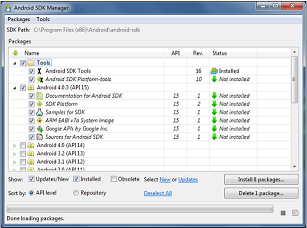
\includegraphics{Packages}
			\caption{Paquetes en SDK Manager}
			\label{fig:SdkManagerPackages}
		\end{figure}
		
	\newpage %Necesario para que la imagen aparezca antes de Firebase
	\subsection{Firebase}
		\begin{itemize}
			\item {\bf Librería}: Añadir la librería de Firebase en el archivo {\it ``build.gradle''} que esta dentro de la carpeta {\it ``app''} en el directorio raíz del proyecto.
				\lstinputlisting[float,language=Java,caption={Importación de la librería de {\it Firebase}},label={code:gradle}]{Code/build.gradle}
				
			\newpage
			\item {\bf Uso}: En los archivos de clase {\it ``java''}\cite{14:java:online} seguir los siguientes pasos:
				\begin{itemize}
					\item {\bf Librerías}: Se han de importar la librerías necesarias:
						\begin{itemize}
							\item {\bf Cliente Firebase}: Importar la librería del cliente.
							\item {\bf Errores Firebase}: Importar la librería de errores en consultas.
							\item {\bf Datos Firebase}: Importar la librería que permite la devolución de datos desde Firebase.
							\item {\bf Consultas Firebase}: Importar la librería para consultas.
							\item {\bf Librería Oyentes}: Importar la librería de los oyentes ({\it ``Listeners''}).
						\end{itemize}
					\item {\bf Contexto}: Añadir el contexto en que se va a usar en la función {\it onCreate}.
					\item {\bf Referencias}: Añadir una referencia a la base de datos o tabla de la misma a la que se van a hacer las consultas.
					\item {\bf Consultas}: Preparar la consulta que se va a hacer.
					\item {\bf Oyentes}: Añadir un oyente ({\it ``Listener''}) a la consulta.
				\end{itemize}
		\end{itemize}
		
		\lstinputlisting[float,language=Java,caption={Ejemplo de uso de {\it Firebase}},label={code:firebase}]{Code/FirebaseExample.java}
		
\newpage		
\section{Tutoriales}
	Antes de comenzar con el desarrollo de la aplicación, se han implementado varios tutoriales para afianzar los conocimientos sobre Android.
	\begin{enumerate}
		\item {\it Build your first app}\cite{29:firstapp:online} %En orden a partir de aquí
		\item {\it Adding the action bar}\cite{30:actionbar:online}
		\item {\it Supporting Different Devices}\cite{31:diferentdevices:online}
		\item {\it Managing the Activity Lifecycle}\cite{32:lifecycle:online}
		\item {\it Building a Dynamic UI with Fragments}\cite{33:fragments:online}
		\item {\it Saving Data}\cite{34:savingdata:online}
		\item {\it Interacting with Other Apps}\cite{35:interacting:online}
		\item {\it Sharing Simple Data}\cite{36:sharingsimpledata:online}
		\item {\it Sharing Files}\cite{37:sharingfiles:online}
		\item {\it Sharing Files with NFC}\cite{38:nfc:online}
		\item {\it Managing Audio Playback}\cite{39:audio:online}
		\item {\it Capturing Photos}\cite{40:photos:online}
		\item {\it Printing Content}\cite{41:printing:online}
		\item {\it Displaying Bitmaps Efficiently}\cite{42:bitmaps:online}
		\item {\it Displaying Graphics with OpenGL ES}\cite{43:opengl:online}
		\item {\it Animating Views Using Scenes and Transitions}\cite{44:transitions:online}
		\item {\it Adding Animations}\cite{45:animations:online}
		\item {\it Connecting Devices Wirelessly}\cite{46:connecting:online}
		\item {\it Performing Network Operations}\cite{47:networks:online}
		\item {\it Syncing to the Cloud}\cite{48:cloud:online}
		\item {\it Transferring Data Using Sync Adapters}\cite{49:adapters:online}
		\item {\it Best Practices for Security \& Privacy}\cite{50:securityprivacity:online}
		\item {\it Best Practices for Testing}\cite{51:testing:online}
		\item {\it Parse}\cite{52:parse:online}
		\item {\it Firebase Storage}\cite{53:firebase:online}
		\item {\it Expandable ListView}\cite{54:expandable:online}
		\item {\it TabHost Swipe}\cite{55:tabhostswipe:online}
		\item {\it ActionBar Tab Swipe}\cite{56:actionbartab:online}
	\end{enumerate}